\documentclass[12pt]{article}
\usepackage[pdfborder={0 0 0.5 [3 2]}, plainpages=false]{hyperref}%
\usepackage[left=1in,right=1in,top=1in,bottom=1in]{geometry}%
\usepackage[shortalphabetic]{amsrefs}%
\usepackage{amsmath}
\usepackage{enumerate}
% \usepackage{enumitem}
\usepackage{amssymb}                
\usepackage{amsmath}                
\usepackage{amsfonts}
\usepackage{amsthm}
\usepackage{bbm}
\usepackage[table,xcdraw]{xcolor}
\usepackage{tikz}
\usepackage{float}
\usepackage{booktabs}
\usepackage{svg}
\usepackage{mathtools}
\usepackage{cool}
\usepackage{url}
\usepackage{graphicx,epsfig}
\usepackage{makecell}
\usepackage{array}

\usepackage[capitalize,nameinlink]{cleveref}
% Per SIAM Style Manual, "section" should be lowercase
\crefname{section}{section}{sections}
\crefname{subsection}{subsection}{subsections}
\Crefname{section}{Section}{Sections}
\Crefname{subsection}{Subsection}{Subsections}

% Per SIAM Style Manual, "Figure" should be spelled out in references
\Crefname{figure}{Figure}{Figures}

% Per SIAM Style Manual, don't say equation in front on an equation.
\crefformat{equation}{\textup{#2(#1)#3}}
\crefrangeformat{equation}{\textup{#3(#1)#4--#5(#2)#6}}
\crefmultiformat{equation}{\textup{#2(#1)#3}}{ and \textup{#2(#1)#3}}
{, \textup{#2(#1)#3}}{, and \textup{#2(#1)#3}}
\crefrangemultiformat{equation}{\textup{#3(#1)#4--#5(#2)#6}}%
{ and \textup{#3(#1)#4--#5(#2)#6}}{, \textup{#3(#1)#4--#5(#2)#6}}{, and \textup{#3(#1)#4--#5(#2)#6}}

% But spell it out at the beginning of a sentence.
\Crefformat{equation}{#2Equation~\textup{(#1)}#3}
\Crefrangeformat{equation}{Equations~\textup{#3(#1)#4--#5(#2)#6}}
\Crefmultiformat{equation}{Equations~\textup{#2(#1)#3}}{ and \textup{#2(#1)#3}}
{, \textup{#2(#1)#3}}{, and \textup{#2(#1)#3}}
\Crefrangemultiformat{equation}{Equations~\textup{#3(#1)#4--#5(#2)#6}}%
{ and \textup{#3(#1)#4--#5(#2)#6}}{, \textup{#3(#1)#4--#5(#2)#6}}{, and \textup{#3(#1)#4--#5(#2)#6}}

% Make number non-italic in any environment.
\crefdefaultlabelformat{#2\textup{#1}#3}

\def\noi{\noindent}
\def\T{{\mathbb T}}
\def\R{{\mathbb R}}
\def\N{{\mathbb N}}
\def\C{{\mathbb C}}
\def\Z{{\mathbb Z}}
\def\P{{\mathbb P}}
\def\E{{\mathbb E}}
\def\Q{\mathbb{Q}}
\def\ind{{\mathbb I}}

\DeclareMathOperator{\spn}{span}
\DeclareMathOperator{\ran}{range}

\graphicspath{ {images/} }

\newtheorem{lemma}{Lemma}
\newtheorem{theorem}{Theorem}
\newtheorem{corollary}{Corollary}
\newtheorem{definition}{Definition}
\newtheorem{proposition}{Proposition}
\newtheorem{hypothesis}{Hypothesis}

\newtheorem{notation}{Notation}

\begin{document}

\section{Mathematical background}

The discrete Klein-Gordon equation (DKG) is given by
\begin{equation}\label{eq:KG}
\partial_t^2 u_n = d (\Delta_2 u)_n - f(u_n)
\end{equation}
where $\Delta_2$ is the discrete second difference operator and $f(u) = V'(u)$ for a smooth potential function $V(u)$. Important versions include the discrete sine-Gordon equation, where $f(u) = -\sin(u)$, and $\phi^4$ variant, where $f(u) = -u(1-u^2)$. The nonlinearity $f(u)$ satisfies the following three properties:
\begin{enumerate}[(i)]
	\item $f(u)$ is an odd function (so $f(0) = 0$) and $f'(0) < 0$
	\item There is a pair of nonzero equilibria $\pm u^*$ with $f(\pm u^*) = 0$ and $f'(u^*) = f'(-u^*) > 0$.
	\item There are no other equilibria in $[-u^*, u^*]$.
\end{enumerate}
We note that the discrete sine-Gordon equation is often written using $f(u) = \sin u$, in which case the pair of equilibria in (ii) are at 0 and $2 \pi$. Equation \cref{eq:KG} is Hamiltonian, with energy given by \cite{KevrekidisWeinstein2000}
\begin{equation}
	\mathcal{H}(u) = \sum_{n=-\infty}^\infty 
	\left( \frac{1}{2} (\partial_t u_n)^2 + \frac{d}{2} (u_{n+1} - u_n)^2 + V(u_n) \right).
\end{equation}

Equilibrium solutions are standing waves which satisfy 
\begin{equation}\label{eq:KGeq}
d (\Delta_2 u)_n - f(u_n) = 0.
\end{equation}
Linearization about such an equilibrium solution $u_n$ yields the eigenvalue problem
\begin{equation}\label{eq:KGevp1}
d (\Delta_2 v)_n - f'(u_n)v_n = \lambda^2 v_n.
\end{equation}
Considered as an eigenvalue problem for $\lambda^2$, the LHS of \cref{eq:KGevp1} is a self-adjoint operator, since it can be represented as a symmetric, infinite dimensional matrix. This implies that $\lambda^2$ is real, which means that $\lambda$ must be either real or pure imaginary. Taking $\omega = \lambda^2$, we re write the eigenvalue problem as
\begin{equation}\label{eq:evp}
d (\Delta_2 v)_n - f'(u_n)v_n = \omega v_n,
\end{equation}
where the eigenvalues are $\lambda = \pm \sqrt{\omega}$.

Using a spatial dynamics approach as in \cite{Parker2020}, let $u_n$ be an equilibrium solution to \cref{eq:KGeq}, and let $U(n) = (u(n), \tilde{u}(n)) = (u_n, u_{n-1})$. Then equation \cref{eq:KGeq} is equivalent to the lattice dynamical system in $\R^2$
\begin{equation}\label{eq:dynEq}
U(n+1) = F(U(n)),
\end{equation}
where
\[
F\begin{pmatrix}u \\ \tilde{u} \end{pmatrix} =
\begin{pmatrix}2u - \tilde{u} + \frac{1}{d}f(u) \\
u
\end{pmatrix}.
\]
This map has three fixed points of interest at $(0,0)$ and $(\pm u^*, \pm u^*)$ (it may in fact have more, depending on the specific form of $f(u)$). For convenience, let $S^\pm = (\pm u^*, \pm u^*)^T$. Linearizing about the fixed points $S^\pm$, we obtain the matrix 
\[
D F(S^\pm)=
\begin{pmatrix}2 + \frac{1}{d}f'(\pm u^*) & -1 \\ 1 & 0
\end{pmatrix}
\]
Since $f'(\pm u^*) > 0$, this has a pair of eigenvalues $\{ r, 1/r \}$ with $r > 0$, where
\[
r = \frac{1}{2d}\left( f'(u^*) + 2d + \sqrt{f'(u^*)(f'(u^*) + 4d)} \right).
\]
Thus $S^\pm$ are hyperbolic saddle equilibria of the lattice dynamical system \cref{eq:dynEq}. We take the existence of a stable, symmetric kink (stationary front) as a hypothesis. From the spatial dynamics perspective, this kink solution a heteroclinic orbit connecting the saddle at $S^-$ to the saddle at $S^+$.

\begin{hypothesis}\label{hyp:kinkexists}
There exists a kink solution $K(n) = (k(n),\tilde{k}(n))$ to \cref{eq:dynEq} which connects the unstable manifold $W^u(-u^*, -u^*)$ and the stable manifold $W^s(u^*, u^*)$. These manifolds intersect transversely in $\R^2$. The kink solution has one of the following odd symmetries:
\begin{itemize}
	\item $k(-n) = -k(n-1)$ (intersite symmetry)
	\item $k(-n) = -k(n)$ (on-site symmetry)
\end{itemize}
Finally, $K(n)$ a ground state kink, i.e. $k(n)$ is a minimizer of the $t$-independent energy functional
\begin{equation}
h[u] = \sum_{n=-\infty}^\infty 
\left( \frac{d}{2} (u_{n+1} - u_n)^2 + V(u_n) \right).
\end{equation}
\end{hypothesis}
Since $K(n)$ is a ground state kink by assumption, it follows that it is spectrally stable \cite{KevrekidisWeinstein2000}. Since the system is Hamiltonian, this implies that the spectrum of the ground state kink lies on the imaginary axis. For specific nonlinearities $f(u)$, including those associated with the discrete sine-Gordon equation and the $\phi^4$ variant, the existence of a symmetric ground state kink is known (see \cite{KevrekidisWeinstein2000} and references therein). For the discrete sine-Gordon equation and the $\phi^4$ variant in particular, the ground state kink has inter-site symmetry. Since $f(u)$ is an odd function, if $u_n$ is a solution to \cref{eq:KGeq}, so is $-u_n$. Thus for every kink solution $K(n)$ to \cref{eq:dynEq} there is a corresponding antikink solution $\tilde{K}(n) = -K(n)$.

The spectrum of the primary kink solution $K(n) = (k(n),\tilde{k}(n))$ can be decomposed into two disjoint sets: the point spectrum consists of isolated eigenvalues for which the corresponding eigenfunction is in $\ell^2(\Z)$, and continuous spectrum is the remaining elements of the spectrum, which consists of bounded, oscillatory modes.Following \cite{KevrekidisWeinstein2000}, the continuous spectrum depends only on the background state of the system and consists of the two symmetric intervals on the imaginary axis
\begin{equation}\label{eq:contspec}
	\sigma_{\text{cont}} = \pm i \left[\sqrt{V''(S^+)}, \sqrt{V''(S^+) + 4d}\right].
\end{equation}
In particular, there is a gap in the continuous spectrum $i\left(-\sqrt{V''(S^+)},\sqrt{V''(S^+)}\right)$ which contain the origin.

Since the discrete Klein-Gordon equation does not possess any continuous symmetries (by contrast with thr continnuum equation, which is translation invariant), there will be no eigenvalues at the origin. Instead, there will be a symmetric pair of eigenvalues, often termed Goldstone modes, which is either real or purely imaginary. For the ground state kink, this pair will be imaginary. For specific nonlinearities $f(u)$, there may be additional eigenvalues, known as internal modes, which lie in the gap in the continuous spectrum. For the ground state kink, these will also be purely imaginary. (See \cite{KevrekidisWeinstein2000}, in particular Figures 2 and 4, for a graphical illustration of the spectrum of the kink solution, including the internal modes, for the discrete sine-Gordon equation and the $\phi^4$ variant).

\section{Multi-kinks}

We can construct multi-kink solutions by joining together an alternating sequence of kinks and anti-kinks in an end-to-end fashion. By the symmetry of $f(u)$, $u_n$ is an equilibrium solution if and only if $-u_n$ is, thus we can always without loss of generality begin with a kink solution. We will characterize a multi-kink in the following way. Let $m > 1$ be the total number of kinks and antikinks. Let $N_i$ ($i = 1, \dots, m-1$) be the distances (in lattice points) between consecutive kinks/anti-kinks. We seek a solution which can be written piecewise in the form 
\begin{equation}\label{eq:Upiecewise}
\begin{aligned}
U_i^-(n) &= c_i K(n) + \tilde{U}_i^-(n) && n \in [-N_{i-1}^-, 0] \\
U_i^+(n) &= c_i K(n) + \tilde{U}_i^+(n) && n \in [0, N_i^+],
\end{aligned}
\end{equation}
where $c_i = (-1)^{i+1}$, $N_i^+ = \lfloor \frac{N_i}{2} \rfloor$, $N_i^- = N_i - N_i^+$, $N_0^- = N_m^+ = \infty$, and
\begin{equation}\label{defN}
N = \frac{1}{2} \min\{ N_i \}.
\end{equation}
The individual pieces are joined together end-to-end as in \cites{Sandstede1998,Parker2020}. The functions $\tilde{K}_i^\pm(n)$ are remainder terms, which we expect to be small. We then have the following theorem.

\begin{theorem}\label{th:KaKexists}
Assume \cref{hyp:kinkexists}. Then there exists a positive integer $N_0$ with the following property. For all $m > 1$ and distances $N_i \geq N_0$, there exists a unique solution $U(n)$ which is composed of $m$ alternating kinks and anti-kinks and can be written piecewise in the form \cref{eq:Upiecewise}. For the remainder terms $\tilde{K}_i^\pm(n)$, we have the estimates
\begin{equation}\label{eq:Westimates}
\begin{aligned}
\|\tilde{U}_i^\pm\| &\leq C r^{-N} \\
| \tilde{U}_i^-(n) | &\leq C r^{-N_{i-1}^-} r^{-(N_{i-1}^- + n)} \\
|\tilde{U}_+^-(n)| &\leq C r^{-N_i^+} r^{-(N_i^+ - n)}
% \tilde{U}_i^+(N_i^+) &= c_{i+1} K(-N_i^-) + \mathcal{O}(r^{-2N}) \\
% \tilde{U}_{i+1}^-(-N_i^-) &= c_i K(N_i^+) + \mathcal{O}(r^{-2N}).
\end{aligned}
\end{equation}
\end{theorem}

For spectral stability, we rewrite the eigenvalue problem \cref{eq:evp} as a lattice dynamical system by taking $V(n) = (v(n), \tilde{v}(n)) = (v_n, v_{n-1})$. Then \cref{eq:evp} is equivalent to the lattice dynamical system in $\R^2$
\begin{equation}\label{eq:EVPdyneq}
V(n+1) = D F( U(n) )V(n) + \omega B V(n),
\end{equation}
where
\[
B = \frac{1}{d}
\begin{pmatrix}1 & 0 \\ 0 & 0
\end{pmatrix}
\] 

STATE STABILITY THEOREMS HERE

\section{Numerical results}

The results we present here are from the discrete sine-Gordon equation
\begin{equation}\label{eq:dSG}
	\partial_t^2 u_n = d (\Delta_2 u)_n + sin(u_n).
\end{equation}
We start by constructing the primary, intersite kink solution $k_n$ by using Matlab for numerical parameter continuation from the anti-continuum (AC) limit ($d = 0$), starting with the solution $(\dots, -\pi, -\pi, \pi, \pi, \dots)$ at the AC limit (\cref{fig:kink}, top left). We then compute the spectrum of the linearization about the primary kink $k_n$ using Matlab's \texttt{eig} function (\cref{fig:kink}, top right).

\begin{figure}[H]
\begin{center}
\begin{tabular}{cc}
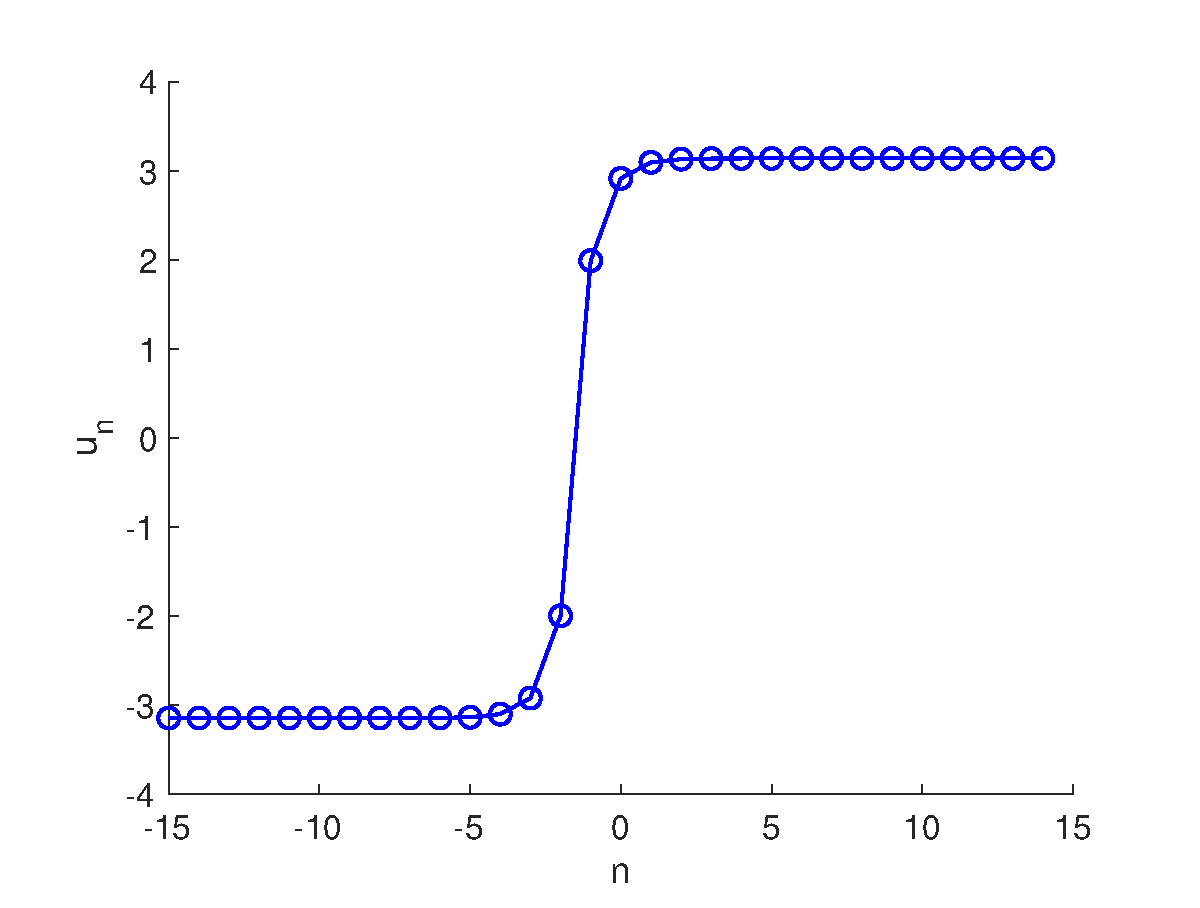
\includegraphics[width=7cm]{1kink.eps}	&
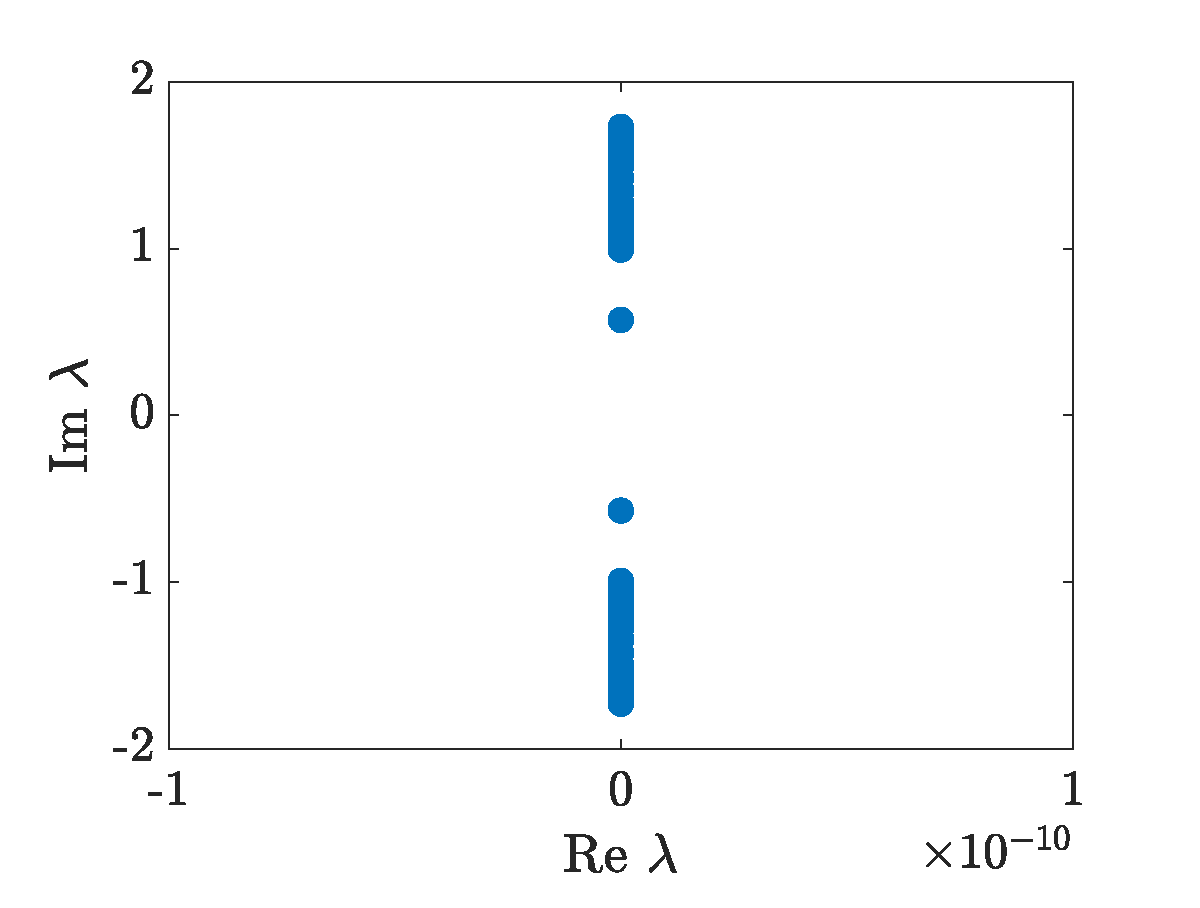
\includegraphics[width=7cm]{1kinkspectrum.eps} \\
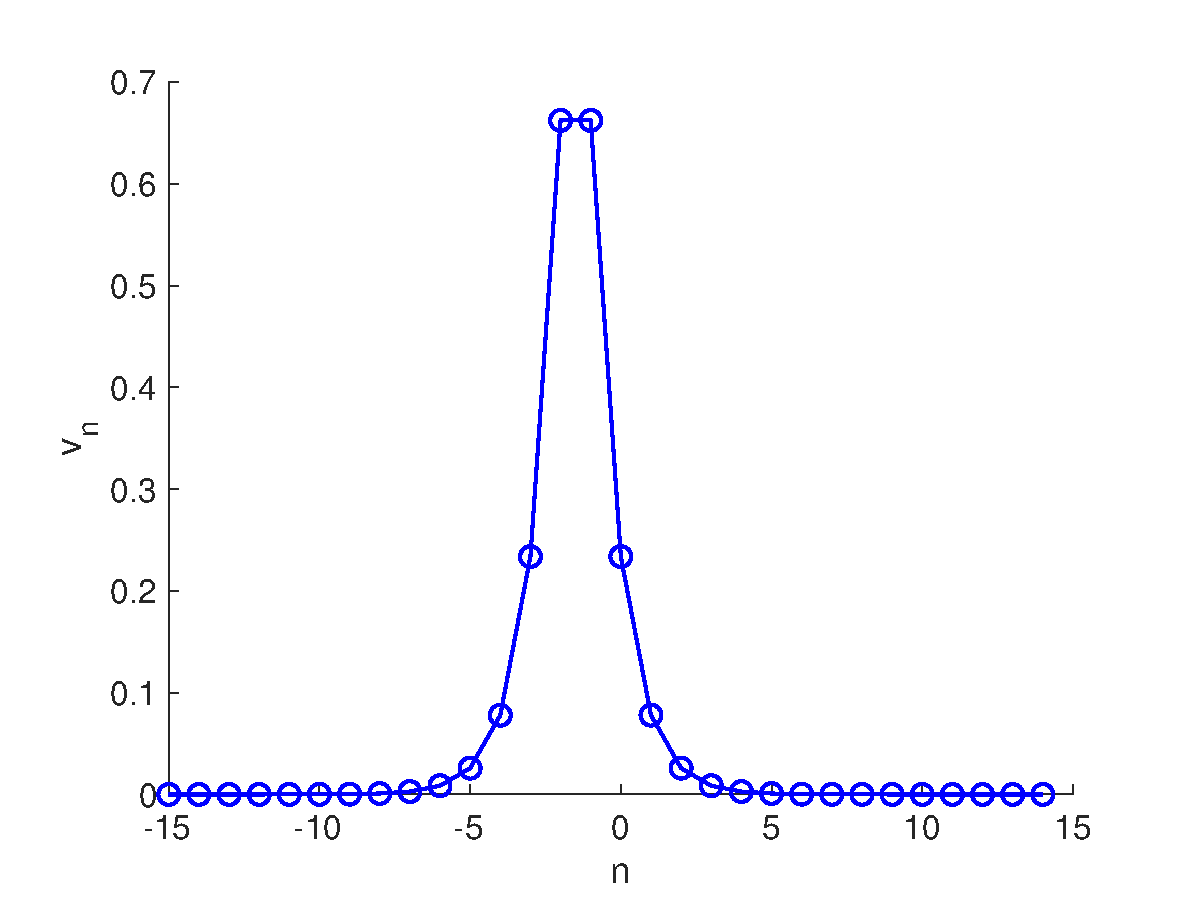
\includegraphics[width=7cm]{1kinkgoldstonemode.eps} &
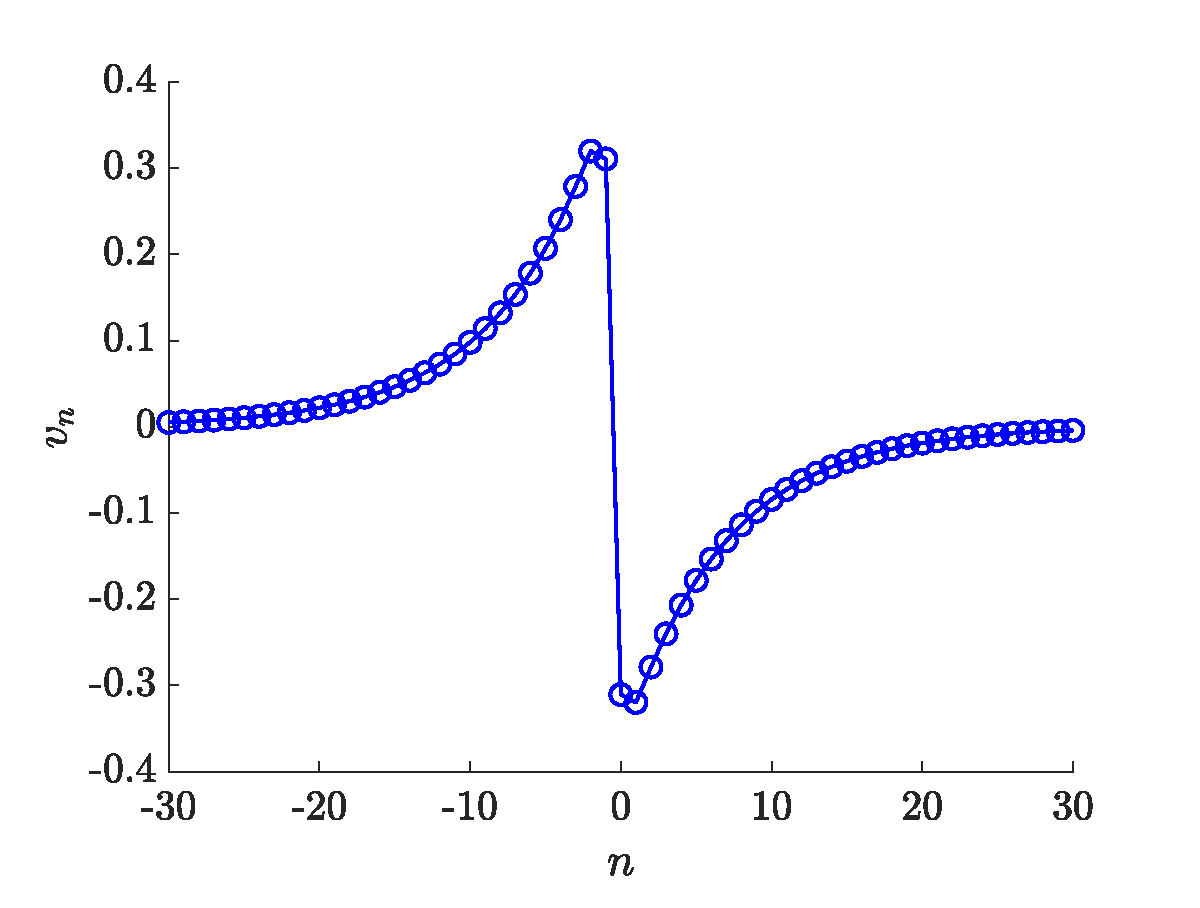
\includegraphics[width=7cm]{1kinkedgemode.eps}
\end{tabular}
\end{center}
\caption{Primary inter-site kink (top left), spectrum of primary kink (top right), Goldstone mode eigenfunction ($\lambda = \pm 0.7789 i$, bottom left), edge mode eigenfunction ($\lambda = \pm 0.9993 i$, bottom left). $d = 0.30$.}
\label{fig:kink}
\end{figure}

The continuous spectrum lies within the interval given by \cref{eq:contspec}, and the pair of Goldstone mode eigenvalues is clearly visible in the continuous spectrum gap. For approximately $d > 0.265$, there is an additional internal mode eigenvalue, known as an edge mode since it arises from the continuous spectrum (see \cite{KevrekidisWeinstein2000}*{Section 2.2}, noting that we are using $d$ in place of $d^2$ in that paper.) The eigenfunctions corresponding to the Goldstone mode and the edge mode are shown in the bottom of \cref{fig:kink}.

\section{Proof of existence results}

The proof is an adaptation of the proofs of Theorems 1 and 3 in \cite{Parker2020}, with one important modification made to gain an improved estimate on the remainder terms $\tilde{U}_i^\pm$. First, we rewrite the system as a fixed point problem. Expanding $F(u)$ in a Taylor series about $c_i K(n)$, we get
\begin{align}\label{eq:Feq1}
F(U_i^\pm(n)) &= F(c_i K(n) + \tilde{U}_i^-(n)) = 
D F(c_i K(n)) \tilde{U}_i^\pm(n) + G(\tilde{U}_i^\pm(n)),
\end{align}
where $G(\tilde{U}_i^\pm(n)) = \mathcal{O}(|\tilde{U}_i^\pm|^2)$ with $G(0) = 0$ and $DG(0) = 0$. Since $f(u)$ is odd, $f'(u)$ is even, thus $D F(c_i K(n)) = D F(K(n))$, and equation \cref{eq:Feq1} becomes
\begin{align}\label{eq:Feq1}
F(U_i^\pm(n)) &= 
D F(K(n)) \tilde{U}_i^\pm(n) + G(\tilde{U}_i^\pm(n).
\end{align}
Since the pieces $U_i^\pm$ in the ansatz \cref{eq:Upiecewise} must match at their endpoints, we obtain the following system of equations for the remainder functions $\tilde{U}_i^\pm$
\begin{align}
\tilde{U}_i^\pm(n+1) &= D F(K(n)) \tilde{U}_i^\pm(n) + G(\tilde{K}_i^\pm(n)) \label{eq:Wsystem1} \\
\tilde{U}_i^+(N_i^+) - \tilde{U}_{i+1}^-(-N_i^-) &= d_i \label{eq:Wsystem2} \\
\tilde{U}_i^+(0) - \tilde{U}_i^-(0) &= 0. \label{eq:Wsystem3}
\end{align}
where
\begin{align}\label{didef}
	d_i &= c_{i+1} K(-N_i^-) - c_i K(N_i^+).
\end{align}
Let $\Phi(m, n)$ be the evolution operators for the linear difference equation 
\[
V(n+1) = D F(K(n)) V(n).
\]
By the stable manifold theorem, $|K(n) - S^+| \leq C r^{-|n|}$ for $n \geq 0$ and $|K(n) - S^-| \leq C r^{-|n|}$ for $n \leq 0$. Since $S^\pm$ are hyperbolic fixed points, we can decompose the evolution operator $\Phi(m, n)$ in exponential dichotomies on $\Z^\pm$ by \cite{Parker2020}*{Lemma 2}. The proof then follows that of \cite{Parker2020}*{Theorems 1 and 3}. Briefly, we write equation \cref{eq:Wsystem1} in fixed-point form using the discrete variation of constants formula together with projections on the stable and unstable subspaces of the exponential dichotomy. The only modification is that we will solve the fixed point equations in function spaces with weighted norms (see \cites{Sandstede1997,ParkerPeriodic} for an example of the same technique in the continuous case). In particular, the remainder functions $\tilde{U}_i^-(n)$ and $\tilde{U}_i^+(n)$ are chosen to be elements of the Banach spaces 
$V^-_{N_{i-1}^-}$ and $V^+_{N_i^+}$, which are defined by
\begin{align*}
	V^-_L &= \left\{ U \in \ell^\infty([-L, 0]) : \| r^{L+n} U(n) \|_{\ell^\infty([-L, 0])} < \infty \right\}\\
	V^+_L &= \left\{ U \in \ell^\infty([0, L]) : \| r^{L-n} U(n) \|_{\ell^\infty([0, L])} < \infty \right\}.
\end{align*}
Aas in \cites{Sandstede1997,ParkerPeriodic}, the fixed point equations are smooth mappings from these weighted function spaces to themselves. As long as $N$ is sufficiently large, we use the implicit function theorem to solve for the remainder functions $\tilde{U}_i^\pm$ as well as the matching conditions \cref{eq:Wsystem2} and \cref{eq:Wsystem3}. Since $W^u(S^-)$ and $W^s(S^+)$ intersect transversely, we have the decomposition $\R^2 = T_{K(0)}W^u(S^-)\oplus T_{K(0)}W^s(S^+)$, thus as in the proof of \cite{Parker2020}*{Theorem 3}, solving \cref{eq:Wsystem3} does not involve jump conditions. The second and third estimates in \cref{eq:Westimates} hold since the estimates on the remainder terms $\tilde{U}_i^\pm$ were obtained in the appropriate weighted space.

\section{Proof of stability results}

For the primary kink $K(n) = (k_n, \tilde{k}_n)$, let $v_0(n)$ be an eigenfunction with corresponding eigenvalue $\lambda_0$, let $\omega_0 = \lambda_0^2$, and let $V_0(n) = (v_0(n), \tilde{v}_0(n)) = (v_0(n), v_0(n-1))$ so that $V_0(n)$ solves the equation
\begin{equation}\label{eq:V0solves}
V_0(n+1) = D F( K(n) )V_0(n) + \omega_0 B V_0(n)
\end{equation}
For the kink-antikink solution $U(n)$, we will take an ansatz which is a piecewise perturbation of $V_0(n)$. Let
\begin{equation}\label{eq:Viansatz}
V_i^\pm(n) = d_i c_i V_0(n) + W_i^\pm(n),
\end{equation}
where $d_i \in \C$ and $c_i = (-1)^{i+1}$. Substituting this into \cref{eq:EVPdyneq} and simplifying using \cref{eq:V0solves}, the eigenvalue problem becomes
\begin{equation}\label{eq:Weq1}
\begin{aligned}
W_i^\pm(n+1)
&= DF(c_i K(n)) W_i^\pm(n) + \omega_0 B W_i^\pm(n) \\
&\qquad + [G_i^\pm(n) + (\omega - \omega_0) B](d_i c_i V_0(n) W_i^\pm(n))
\end{aligned}
\end{equation}
where
\[
G_i^\pm(n) = DF(U_i^\pm(n)) - DF(c_i K(n)).
\]
Let 
\[
A_i(n; \omega_0) = DF(c_i K(n)) + \omega_0 B
\]
Then \cref{eq:Weq1} becomes
\begin{align}\label{eq:Weq2}
W_i^\pm(n+1)
&= A_i(n; \omega_0) W_i^\pm(n) + [G_i^\pm(n) + (\omega - \omega_0) B](d_i c_i V_0(n) + W_i^\pm(n)).
\end{align}

As long as $|\omega_0| < f'(\pm u*)$ (WHICH WE SHOULD BE ABLE TO SHOW OR CAN ASSUME, IN ANY CASE IT IS REASONABLE GIVEN TYPICAL $f)$), $A_i(n)$ is exponentially asymptotic to a constant matrix with an exponential dichotomy, so it has one as well. WE CAN NOW USE ALL THE EXPONENTIAL DICHOTOMY TRICKS WE KNOW.

In addition to solving \cref{eq:Weq2}, the eigenfunction must satisfy matching conditions at $n = \pm N_i$ and $n = 0$. Thus the system of equations we need to solve is
\begin{equation}\label{eq:eigWsystem1}
\begin{aligned}
& W_i^\pm(n+1)
= A_i(n; \omega_0) W_i^\pm(n) + [G_i^\pm(n) + (\omega - \omega_0) B](d_i c_i V_0(n) + W_i^\pm(n))\\
& W_i^+(N_i^+) - W_{i+1}^-(-N_i^-) &= D_i d \\
& W_i^+(0) - W_i^-(0) = 0,
\end{aligned}
\end{equation}
where
\begin{equation}\label{defDid}
D_i d = d_{i+1} c_{i+1} V_0(-N_i^-) - d_i c_i V_0(N_i^+)
\end{equation}

Things to note:
\begin{itemize}
\item Equation $V(n+1) = A(n; \lambda_0)$ has unique bounded solution $V_0(n) = (v_0(n), v_0(n-1))$. Let $\Phi(m, n; \lambda_0)$ be the evolution operator for this.
\item Adjoint equation $Z(n) = A(n; \lambda_0)^* Z(n+1)$ has unique bounded solution $Z_0(n) = (-v_0(n-1), v_0(n))$ which is orthogonal to $Z_0(n)$. (This uses the fact that $\lambda_0$ is real or pure imaginary when we take the adjoint).
\item $A(n; \lambda_0)$ is exponentially asymptotic (on both ends) to a hyperbolic matrix $A_0$ with 1-dimensional stable and unstable eigenspaces $E^s$ and $E^u$ with corresponding projections $P_0^s$ and $P_0^u$.
\item Because of this, $V(n+1) = A(n; \lambda_0)$ induces an exponential dichotomy on $\Z^\pm$.
\end{itemize}

Since $\R^2 = \spn\{ V_0(0), Z_0(0) \}$, we can rewrite our system as 

\begin{equation}\label{eq:eigWsystem2}
\begin{aligned}
&W_i^\pm(n+1)
= A_i(n; \omega_0) W_i^\pm(n) + [G_i^\pm(n) + (\omega - \omega_0) B](d_i c_i V_0(n) + W_i^\pm(n))\\
&W_i^+(N_i^+) - W_{i+1}^-(-N_i^-) = D_i d \\
&W_i^+(0) - W_i^-(0) \in \C Z_0(n),
\end{aligned}
\end{equation}
with jump conditions
\begin{equation}
\langle Z_0(n), W_i^+(0) - W_i^-(0) \rangle = 0
\end{equation}

As in \cite{Sandstede1998}, we write equation \cref{eq:Weq1} as a fixed point problem using the discrete variation of constants formula together with projections on the stable and unstable subspaces of the exponential dichotomy. Let $\delta > 0$ be small, and choose $N$ sufficiently large so that $r^{-N} < \delta$. Define the spaces
\begin{align*}
V_W &= \ell^\infty([-N_{i-1}, 0]) \oplus \ell^\infty([0, N_i])  \\
V_a &= \bigoplus_{i=0}^{n-1} E^u \oplus E^s \\
V_b &= \bigoplus_{i=0}^{n-1} \ran P_-^u(0) \oplus \ran P_+^s(0)\\
V_\lambda &= B_\delta(\lambda_0) \subset \C \\
V_d &= \C^d.
\end{align*}
Then for
\begin{align*}
W = (W_i^-, W_i^+) &\in V_W \\
a = (a_i^-, a_i^+) &\in V_a \\
b = (b_i^-, b_i^+) &\in V_b \\
\lambda &\in V_\lambda,
\end{align*}
the fixed point equations for the eigenvalue problem are
\begin{equation}\label{fpeig}
\begin{aligned}
W_i^-(n) &= 
\Phi_s^-(n, -N_{i-1}^-) a_{i-1}^- + \sum_{j = -N_{i-1}^-}^{n-1} \Phi_s^-(n, j+1)
[G_i^-(j) + (\omega - \omega_0) B](d_i c_i V_0(j) + W_i^-(j))
 \\
&+ \Phi_u^-(n, 0) b_i^- - \sum_{j = n}^{-1} \Phi_u^-(n, j+1) 
[G_i^-(j) + (\omega - \omega_0) B](d_i c_i V_0(j) + W_i^-(j))\\
W_i^+(n) &= \Phi_s^+(n, 0; \theta_i) b_i^+ + \sum_{j = 0}^{n-1} \Phi_s^+(n, j+1) 
[G_i^+(j) + (\omega - \omega_0) B](d_i c_i V_0(j) + W_i^+(j))\\
&+ \Phi_u^+(n, N_i^+) a_i^+ - \sum_{j = n}^{N_i^+-1} \Phi_u^+(n, j+1) 
[G_i^+(j) + (\omega - \omega_0) B](d_i c_i V_0(j) + W_i^+(j)),
\end{aligned}
\end{equation}
where $a_0^- = a_m^+ = 0$ and the sums are defined to be $0$ if the upper index is smaller than the lower index.

We now follow the procedure and invert the system \cref{eq:eigWsystem2} in the following steps.

\begin{enumerate}
\item Solve for the remainder functions $W_i^\pm(n)$
\item Use the second equation in \cref{eq:eigWsystem2} to solve for the $a_i^\pm$
\item Use the third equation in \cref{eq:eigWsystem2} to solve for the $b_i^\pm$
\item Evaluate the jump conditions
\end{enumerate}

At the end of the day, we should have
\begin{align*}
a_i^+ &= P_0^u D_i d + \text{``h.o.t.''} \\
a_i^- &= -P_0^s D_i d + \text{``h.o.t.''}
\end{align*}
When we compute the jump conditions, the only terms that should contribute are the ones with $a_i^\pm$ (tail interactions) and the sum involving $(\omega - \omega_0) B (d_i c_i V_0(j)$ (Melnikov-type sum). Putting all of this together, the jump conditions should be, to leading order, 
\begin{equation}\label{eq:xieq}
\begin{aligned}
\xi_i = \langle &Z_0(N_i^+), P_0^u D_i d \rangle 
+ \langle Z_0(-N_{i-1}^-), P_0^s D_{i-1} d \rangle 
- (\omega - \omega_0) d_i c_i \sum_{j = -\infty}^{\infty} \langle Z_0(j+1), B V_0(j)\rangle
\end{aligned}
\end{equation}
For the terms in the Melnikov sum,
\[
\langle Z_0(j+1), B V_0(j)\rangle = \frac{1}{d} \langle (-v_0(j), v_0(j-1))^T, (v_0(j), 0) \rangle
= -\frac{1}{d}v_0(j)^2,
\]
which means the Melnikov sum will be given by
\begin{equation}\label{eq:M}
M = \sum_{j = -\infty}^{\infty} v_0(j)^2 = \| v_0 \|_{\ell^2},
\end{equation}
which is always positive. For the other terms, we note that
\begin{align*}
P_0^u D_i d &= d_{i+1} c_{i+1} V_0(-N_i^-) + \text{``h.o.t.''} \\
P_0^s D_i d &= -d_i c_i V_0(N_i^+) + \text{``h.o.t.''}
\end{align*}
Putting all of this together, we have, to leading order,
\begin{align*}
\xi_i = \langle Z_0(N_i^+), V_0(-N_i^-) \rangle d_{i+1} c_{i+1}
- \langle Z_0(-N_{i-1}^-), V_0(N_{i-1}^+) \rangle d_{i-1} c_{i-1}
+ \dfrac{1}{d} (\omega - \omega_0) d_i c_i M
\end{align*}
Since $c_i$ and $c_{i+1}$ have opposite signs, this simplifies to 
\begin{align*}
\xi_i = \langle Z_0(N_i^+), V_0(-N_i^-) \rangle d_{i+1}
- \langle Z_0(-N_{i-1}^-), V_0(N_{i-1}^+) \rangle d_{i-1}
- \dfrac{1}{d} (\omega - \omega_0) d_i M
\end{align*}
Let
\begin{align*}
a_i &= \langle Z_0(N_i^+), V_0(-N_i^-) \rangle 
= v_0(N_i^+)v_0(-N_i^- - 1) - v_0(N_i^+ - 1)v_0(-N_i^-)
\end{align*}
Then
\[
\langle Z_0(-N_i^-), V_0(N_i^+) \rangle 
= v_0(N_i^+ - 1)v_0(-N_i^-) - v_0(N_i^+)v_0(-N_i^- - 1) = -a_i
\]
Thus we have
\begin{align*}
\xi_i = a_i d_{i+1}
+ a_{i-1} d_{i-1}
- \dfrac{1}{d} (\omega - \omega_0) d_i M
\end{align*}
The $a_i$ can be simplified based on symmetries of the eigenfunction $v_0(n)$. For even eigenfunctions, we have $v_0(-n) = v_0(n-1)$, (the Goldstone mode, appears to be even), so we have
\begin{align}\label{eq:ai}
a_i = v_0(N_i^+)v_0(N_i^-) - v_0(N_i^+ - 1)v_0(N_i^- -1)
\end{align}


\bibliographystyle{amsplain}
\bibliography{DKG.bib}

\end{document}